\begin{pastexam}[label={px:nccu-115-dsa-01}]{政大資科所 115 學年度 第 1 題}
（單選）

(5\%) What is the upper bound on the height of a red-black tree with $n$ internal nodes?

(A)~$n/2$ \qquad (B)~$\log_2(n+1)$ \qquad (C)~$n$ \qquad (D)~$2\log_2(n+1)$
\end{pastexam}

\begin{pastsoln}
答案是 (D)。

資結書定理~10.4：有 $n$ 個內部節點的紅黑樹，高度 $h \le 2\lg(n+1)$。 理由是從根往下的任一條路徑上，
紅色節點不會相連，所以最長的路徑上黑色節點至少佔一半，根的黑高度 $\mathrm{bh} \ge h/2$；而黑高度
$\mathrm{bh}$ 的子樹至少有 $2^{\mathrm{bh}} - 1$ 個內部節點（資結書引理~10.3），得到
$n \ge 2^{h/2} - 1$，移項取對數就是 $h \le 2\log_2(n+1)$。

逐項檢查：
\begin{itemize}
\item (A) $n/2$：$n = 1$ 時樹只有根，高度是 $1$，已經超過 $1/2$，不是上界；$n$ 大的時候它又遠大於
$2\log_2(n+1)$，就算成立也不是題目要的那個界。 錯。
\item (B) $\log_2(n+1)$：這是「完全平衡」的二元樹才有的高度，紅黑樹允許最長路徑是最短路徑的兩倍，
會超過它。 例如下面這棵 $n = 6$ 的紅黑樹（白底是紅色節點，灰底是黑色節點）：根和根的左兒子是黑色；
根的右兒子是紅色，它的兩個兒子是黑色；右邊那個黑色兒子再掛一個紅色的右兒子。 每條從根到 NIL 的路徑都
經過 $2$ 個黑色節點，紅色節點的兒子都是黑色，所以是合法的紅黑樹。 最長路徑從根往右走經過 $4$ 個節點
（$3$ 條邊），而 $\log_2 7 \approx 2.81$，不管高度用節點數還是邊數算都超過。 錯。
\begin{center}
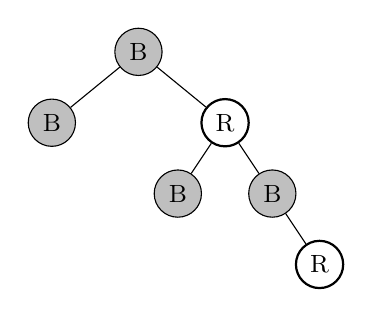
\begin{tikzpicture}[level distance=9mm,
  level 1/.style={sibling distance=22mm}, level 2/.style={sibling distance=12mm},
  b/.style={circle,draw,fill=black!25,minimum size=6mm,inner sep=0pt,font=\small},
  r/.style={circle,draw,thick,minimum size=6mm,inner sep=0pt,font=\small}]
\node[b] {B}
  child {node[b] {B}}
  child {node[r] {R}
    child {node[b] {B}}
    child {node[b] {B}
      child[missing] {}
      child {node[r] {R}}}};
\end{tikzpicture}
\end{center}
\item (C) $n$：任何 $n$ 個節點的二元樹高度都不超過 $n$，這句話成立，但它沒有用到紅黑樹的性質，
紅黑樹的意義正是把高度壓到 $O(\log n)$。 題目要的是紅黑樹的上界，不選。
\item (D) $2\log_2(n+1)$：就是上面的定理。 對。
\end{itemize}
\end{pastsoln}
